\section{Process' Perspective}
\label{ch:background} 

\subsection{CI/CD pipeline using GitHub actions}
%A complete description of stages and tools included in the CI/CD chains, including deployment and release of your systems.
Our overall workflow is shown in Figure \ref{fig:activity_diagram}.
%TC:ignore
\begin{figure}[h]
      \centering
      \makebox[\linewidth]{
      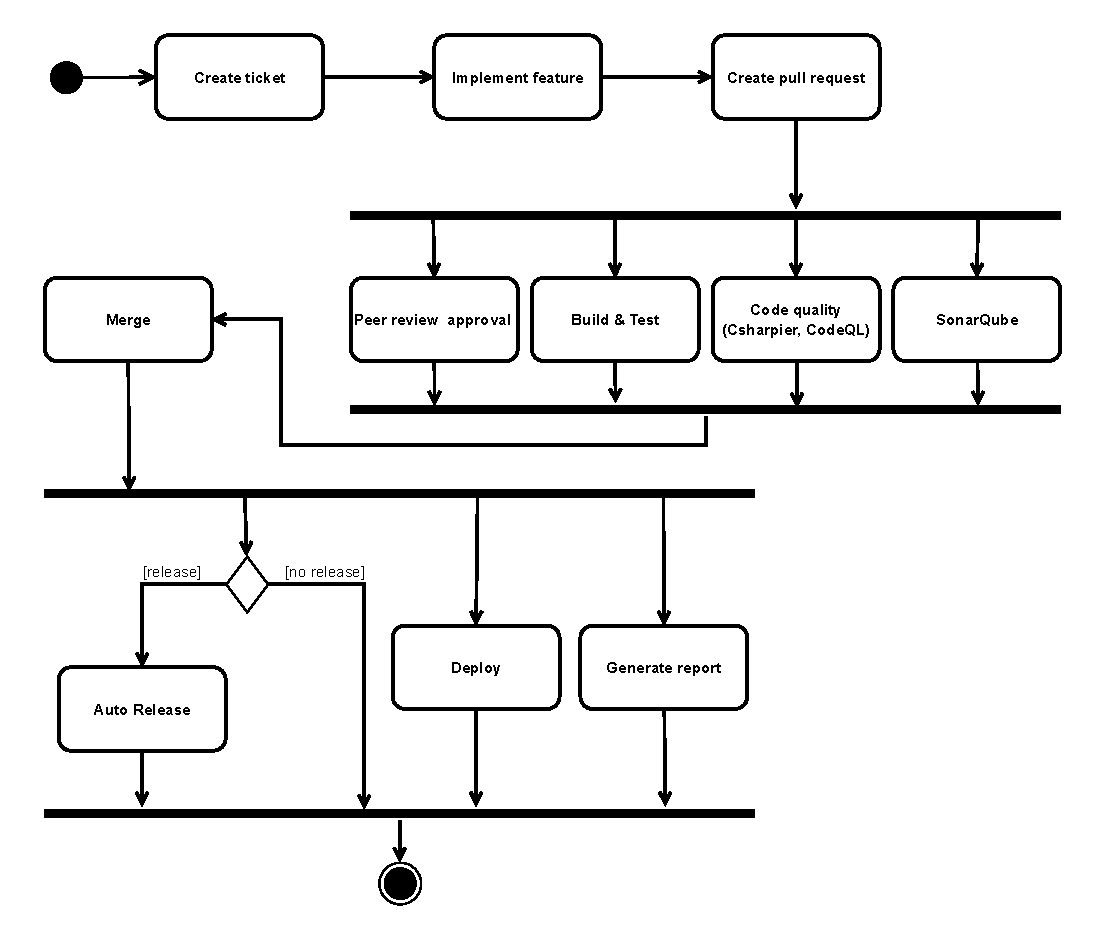
\includegraphics[width=1.4\textwidth]{images/activity_diagram.drawio.pdf}}
      \caption{Activity diagram of the CI/CD pipeline}
      \label{fig:activity_diagram}
\end{figure}
%TC:endignore

We use \texttt{GitHub Issues} to create tickets.
The \texttt{CI/CD} pipeline is implemented using \texttt{GitHub Actions} 
to automate building, testing, code quality analysis, releasing, 
and deployment of the \texttt{MiniTwit} application.

\subsubsection{Build and Test Workflow}
This workflow is triggered on every pull request (\texttt{PR}) to \texttt{main}.
The purpose of this is to build the application, run tests, 
and generate a code coverage report.
Passing this workflow is a requirement for merging 
\texttt{PR}'s into \texttt{main}.

\subsubsection{Code Quality Workflow}
This workflow makes use of \texttt{GitHub}'s \texttt{CodeQL}\cite{codeql} 
to perform static code analysis of \texttt{C\#} code.
It uses the same triggers as the build and test workflow.
Before performing the analysis, it formats the \texttt{C\#} code using 
\texttt{csharpier}\cite{csharpier}.
It then performs a semantic code analysis to find security 
vulnerabilities and displays the results on the \texttt{PR}'s.
It once discovered that we leaked a third-party secret 
in our code, which we then removed and updated.

Additionally, we use \texttt{SonarQube}\cite{sonarqube}, 
\texttt{CodeFactor}\cite{codefactor}, and \texttt{OpenSSF}\cite{Openssf} 
to perform code analysis such as code coverage, duplication, 
security risks, and other good practices.
The results are displayed on the front page of the repository 
on \texttt{GitHub} as badges.

\subsubsection{Auto Merge Dependabot Workflow}
Our project uses \texttt{dependabot} to automatically update
dependencies in the project.
We have a \texttt{GitHub Action} that detects \texttt{PR}'s 
created by \texttt{dependabot}, and automatically merges 
them into \texttt{main} if all workflows pass.
This ensures that we have the latest dependencies,
and we avoid having to manually merge \texttt{dependabot} 
\texttt{PR}'s.

\subsubsection{Auto Release Workflow}
This workflow is triggered on every push to the 
\texttt{main} branch, and automatically 
creates a new release on \texttt{GitHub} if it has
a commit message in the format \texttt{Release: x.y}. 
Here \texttt{x} and \texttt{y} are the major and minor version numbers, respectively.
Release information such as title and updates, should be added to the file \texttt{CHANGELOG.md}.

\subsubsection{Deployment Workflow}
This workflow is triggered on a push to \texttt{main}.
It is responsible for building \texttt{Docker images}, 
uploading, and deploying them to \texttt{Digital Ocean} droplets.
It uses \texttt{Docker Hub} to push the built images.
Then it uses \texttt{scp} and \texttt{ssh} to copy remote files 
to the relevant droplets, which are then executed to 
deploy the application. For deployment safeguards,
\texttt{SSH} keys, \texttt{IP} addresses, and credentials are stored in \texttt{GitHub Secrets},
which are then used in the workflows to access the \texttt{Digital Ocean} droplets and to 
authenticate with \texttt{Docker Hub}.


\subsection{Terraform}
\texttt{Terraform} is used to provision and manage our infrastructure as code, 
to automatically set up droplets in \texttt{Digital Ocean}. 
The result of the \texttt{Terraform} setup is illustrated 
in Figure \ref{fig:deployment_diagram}.
\texttt{Terraform} creates all droplets with \texttt{SSH} keys and files.
It also configures the \texttt{Docker Swarm} for the \texttt{API}.
It then calls the deploy scripts on each droplet.
Finally, it assigns the reserved \texttt{IP}'s.
The \texttt{Terraform} state file is shared in the remote \texttt{Digital Ocean Spaces}.

\subsection{Security assessment}
To analyse security risks in our code, 
we use tools like \texttt{GitHub}'s \texttt{CodeQL}\cite{codeql} that 
integrates with our \texttt{CI/CD} pipeline.
This provides a display of security vulnerabilities in our code,
which is shown on the \texttt{PR}'s.

To analyse security risks of \texttt{Docker images}, \texttt{Docker Scout} has been used to get
quick overviews of security risks from our \texttt{Docker images}.
It scores the images in four levels: \texttt{low}, \texttt{medium}, \texttt{high}, and \texttt{critical}.
Additionally, it provides recommendations on how to fix the issues.

We use a risk assessment matrix to assess the probability and impact of security risks. 
These are split into: probability (\texttt{unlikely}, \texttt{possible}, \texttt{likely}) 
and impact (\texttt{negligible}, \texttt{moderate}, and \texttt{catastrophic}).
The result is shown in Table \ref{tab:risk_matrix}.
%TC:ignore
\begin{table}[H]
\caption{Risk assessment matrix}
\vspace{0.3cm}
\label{tab:risk_matrix}
\begin{tabular}{ll|lll|}
\cline{3-5}
    &      & \multicolumn{3}{c|}{\cellcolor[HTML]{BBBBBB}Possibility of risk} \\ \cline{2-5} 
\multicolumn{1}{l|}{}     &      & \multicolumn{1}{l|}{Unlikely} & \multicolumn{1}{l|}{Possible}  & Likely  \\ \hline
\multicolumn{1}{|l|}{\cellcolor[HTML]{BBBBBB}}  & Catastrophic  & \multicolumn{1}{l|}{\cellcolor[HTML]{E0D050}\begin{tabular}[c]{@{}l@{}}Access to the \\database\end{tabular}}   & \multicolumn{1}{l|}{\cellcolor[HTML]{E07070}\begin{tabular}[c]{@{}l@{}}Leak of secrets\\ \& Droplet failure\end{tabular} } & \cellcolor[HTML]{E07070} \\ \cline{2-5} 
\multicolumn{1}{|l|}{\cellcolor[HTML]{BBBBBB}}  & Moderate & \multicolumn{1}{l|}{\cellcolor[HTML]{70D080}}    & \multicolumn{1}{l|}{\cellcolor[HTML]{E0D050}\begin{tabular}[c]{@{}l@{}}Overloading the \\API with requests\end{tabular}} &\cellcolor[HTML]{E07070}\begin{tabular}[c]{@{}l@{}}Login credentials\\leaked\end{tabular} \\ \cline{2-5} 
\multicolumn{1}{|l|}{\multirow{-3}{*}{\cellcolor[HTML]{BBBBBB}\begin{tabular}[c]{@{}l@{}}Impact\\ of risk\end{tabular}}}            & Negligible & \multicolumn{1}{l|}{\cellcolor[HTML]{70D080}}    & \multicolumn{1}{l|}{\cellcolor[HTML]{70D080}}  & \cellcolor[HTML]{E0D050}Access to Seq     \\ \hline
\end{tabular}
\end{table}
%TC:endignore

For details about each risk scenario see Appendix \ref{appn:B}.

\subsection{Scaling}
The \texttt{Client} uses Blazor WebAssembly (\texttt{WASM}) for client-side redering, 
avoiding server-side rendering.
The application logic is executed in the browser, and only lightweight 
\texttt{JSON} requests are made to the \texttt{API} to fetch data.
This results in a heavly initial load for the user, as the entire application is downloaded 
locally, however afterwards, 
this setup offers high responsiveness and scalability by addtionally using 
a \texttt{Hybrid Cache}.
To overcome the browser caching limitations (e.g. 16 GB and frequently disks 
reads), we could introduce a \texttt{Redis} cache to potentially support 
infinite and more efficient caching.

The \texttt{API} is scalable as it is stateless and uses \texttt{Docker Swarm}, 
allowing horizontal scaling of both manager and worker nodes.
The \texttt{database} is not currently optimized in terms of scalability, 
as it is a single instance of \texttt{PostgreSQL}.
The database is the potential bottleneck of the system, as it is the only shared 
resource between the \texttt{API} nodes.
To fix this, we could use sharding to distribute the load of the \texttt{Database} 
across multiple instances.
By splitting the \texttt{database} into multiple shards, we can distribute 
the load of the \texttt{API} across multiple \texttt{PostgreSQL} instances.
This could introduce some complexity and overhead, as it would be harder 
to manage and query the data.

\subsection{AI-assistants}

In general we use \texttt{CoPilot} to autocomplete code.
We used \texttt{ChatGPT} and other chat bots to help
with especially bash script files and converting 
the \texttt{Python} application to \texttt{C\#}.

When we were setting up \texttt{Vagrant} 
(which was later replaced by \texttt{Terraform}),
we used \texttt{ChatGPT} to try and debug an error we had with 
the database migration. However, we could not get it 
to detect what was wrong, and we ended up solving it ourselves.
